\documentclass[11pt,letterpaper]{article}
\usepackage[lmargin=1in,rmargin=1in,tmargin=1in,bmargin=1in]{geometry}
\usepackage{../style/homework}
\usepackage{../style/commands}
\setbool{quotetype}{false} % True: Side; False: Under
\setbool{hideans}{false} % Student: True; Instructor: False

% -------------------
% Content
% -------------------
\begin{document}

\homework{2: Due 02/06}{There is only one boss. The customer. And he can fire everybody in the company from the chairman on down, simply by spending his money somewhere else.}{Sam Walton}

% Problem 1
\problem{10} Suppose that the revenue and cost function for a certain item are given by $R(q)= 199.99q$ and $C(q)= 56.24q + 1260000$, respectively. 
	\begin{enumerate}[(a)]
	\item How much does the company sell each item for? How much does it cost to make each item?
	\item What are the fixed costs for the production of this good?
	\item What is the profit or loss if the company produces and sells five-thousand of these items?
	\item What is the break-even point? At least many items does this company need to sell in order to make a profit on this item?
	\end{enumerate} 

\sol 
\begin{enumerate}[(a)]
\item The function $R(q)= 199.99q= 199.99q + 0$ is linear, i.e. has the form $y= mx + b$ with $R= y$, $q= x$, $m= 199.99$, and $b= 0$. Therefore, the rate of change of $R(q)$ is constant. The rate of change of $R(q)$ is the sales amount of each item. Therefore, each item sells for \$199.99. Because the function $C(q)= 56.24q + 1260000$ is linear, i.e. has the form $y= mx + b$ with $C= y$, $q= x$, $m= 56.24$, and $b= 1260000$, the rate of change of $C(q)$ is constant. The rate of change of $C(q)$ is the cost of each item. Therefore, each item costs \$56.24 to produce. \pspace

\item The fixed costs are the costs not associated with production of the good/service. But then this must be the cost when no items are produced, i.e. $C(0)$. We have $C(0)= 56.24(0) + 1260000= 1260000$. Therefore, the fixed costs are \$1,260,000. \pspace

\item The profit function is given by $P(q)= R(q) - C(q)$. But this is\dots
	\[
	P(q)= R(q) - C(q)= 199.99q - (56.24q + 1260000)= 199.99q - 56.24q - 1260000= 143.75q - 1260000
	\]
Therefore, we have $P(5000)= 143.75(5000) - 1260000= 718750 - 1260000= -\$541250$. But then the company has a deficit of \$541,250. Alternatively, we have $R(5000)= \$999950$ and $C(5000)= \$1541200$. Then the profit is $\$999950 - \$1541200= -\$541250$, i.e. a deficit of \$541,250. \pspace

\item The break-even point is the point where revenue equals cost, i.e. $R(q)= C(q)$. Alternatively, this is the point where $P(q)= 0$. But then we have\dots
	\[
	\begin{aligned}
	P(q)&= 0 \\[0.3cm]
	143.75q &- 1260000= 0 \\[0.3cm]
	143.75q&= 1260000 \\[0.3cm]
	q&= 8765.22
	\end{aligned}
	\]
Therefore, the company must produce/sell at least 8,766~items to turn a profit. 
\end{enumerate}



\newpage



% Problem 2
\problem{10} Bread Pitt is a bread and pastry shop. They make an exquisite challah bread that is a talk of the town and sells for only \$7.49. The cost to make each loaf is approximately \$0.89. However, between the utilities and various other costs, the shop pays at least \$847 per day just to stay open. 
	\begin{enumerate}[(a)]
	\item What are the fixed and variable costs for producing this bread?
	\item Find the cost function for this bread.
	\item Find the revenue function for this bread.
	\item Find the break-even point for producing this challah bread. 
	\end{enumerate} \pspace

\sol 
\begin{enumerate}[(a)]
\item The fixed costs are the cost of production that do not change based on the amount of production. Here, this is the \$847 cost of keeping the business open each day. The variables costs vary with the production level. Because each bread loaf costs \$0.89 to produce, if $q$ loaves are made, the variable costs are $0.89q$ for those loaves. \pspace

\item We know the costs are the sum of the fixed and variable costs. But then $C(q)= 0.89q + 847$. \pspace

\item Because the shop sells each loaf for \$7.49, if they sell $q$ loaves, they make $7.49q$ for selling those loaves. Therefore, $R(q)= 7.49q$. \pspace

\item The break-even point is the point where revenue equals cost. But then we have\dots
	\[
	\begin{aligned}
	R(q)&= C(q) \\[0.3cm]
	7.49q&= 0.89q + 847 \\[0.3cm]
	6.60q&= 874 \\[0.3cm]
	q&= 132.42
	\end{aligned}
	\]
Therefore, the shop need sell at least 133~loaves to turn a profit. 
\end{enumerate}



\newpage



% Problem 3
\problem{10} Suppose a company produces two items, $q_1$ and $q_2$, and has a cost function given by $C(q_1, q_2)= 746.12q_1 + 646.95q_2 + 846221$. 
	\begin{enumerate}[(a)]
	\item What are the fixed costs for producing these two items?
	\item What is the total cost associated with producing 20 of the first item and 25 of the second item?
	\item How much does it cost to produce the first item? How much does it cost to produce the second item?
	\end{enumerate} \pspace

\sol 
\begin{enumerate}[(a)]
\item The fixed costs are the costs associated with production which do not depend on the level of production. But this is precisely the cost $C(0, 0)$. We have $C(0, 0)= 0 + 0 + 846221= 846221$. Therefore, the fixed costs are \$846,221. \pspace

\item This is\dots
	\[
	C(20, 25)= 746.12(20) + 646.95(25) + 846221= 14922.40 + 16173.80 + 846221= \$877,317.2
	\] \pspace

\item From the function $C(q_1, q_2)$, we can see that it costs $\$746.12$ to produce the first item and $\$646.95$ to produce the second item. 
\end{enumerate}



\newpage



% Problem 4
\problem{10} Suppose that you have a revenue function given by $R(q)= 20q$ and a cost function given by $C(q)= 5q + 160$. 
	\begin{enumerate}[(a)]
	\item Without finding the profit function, find the break-even point for the production/sale of this item.
	\item Sketch the revenue and cost function on the plot below. 
	\item Without finding the profit function, explain using (b) where the profit function will cross the $q$-axis. 
	\item Find the profit function and show that it has the $q$-intercept you found in (c). 
	\end{enumerate} \pspace

\sol 
\begin{enumerate}[(a)]
\item The break-even point is the point where revenue equals cost. But then we have\dots
	\[
	\begin{aligned}
	R(q)&= C(q) \\[0.3cm]
	20q&= 5q + 160 \\[0.3cm]
	15q&= 160 \\[0.3cm]
	q&= 10.6667
	\end{aligned}
	\] 

\item The revenue function $R(q)= 20q$ is linear with slope 20 and $y$-intercept 0. The function $C(q)= 5q + 160$ is linear with slope 5 and $y$-intercept 160. Using this, we plot $R(q)$ and $C(q)$ on the plot below. \pspace

\item We know the break-even point is when the profit is $0$, i.e. when $P(q)= 0$. But this is a $q$-intercept for $P(q)$. Therefore, $P(q)$ will cross the $q$-axis at $q= 10.6667$. 


\item We know that $P(q)= R(q) - C(q)= 20q - (5q + 160)= 20q - 5q - 160= 15q - 160$. The $q$-intercept of $P(q)$ is when $P(q)=0 $. But then we have $15q - 160= 0$ so that $15q= 160$. This implies $q= 10.6667$, which confirms the work above. 
\end{enumerate}

	\vfill
	
	\[
	\fbox{
	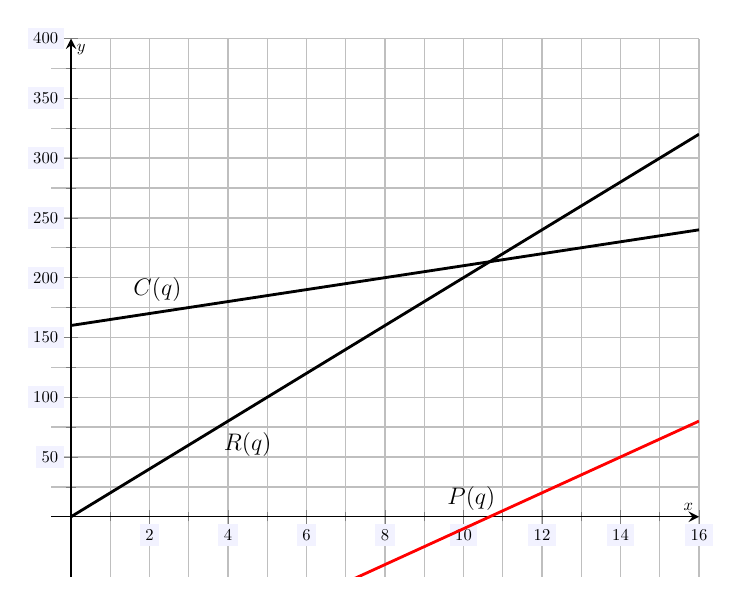
\begin{tikzpicture}[scale=1.2,every node/.style={scale=0.5}]
	\begin{axis}[
	grid=both,
	axis lines=middle,
	ticklabel style={fill=blue!5!white},
	xmin= -0.5, xmax=16,
	ymin= -50, ymax=400,
	xtick={0,2,...,16},
	ytick={0,50,...,400},
	minor x tick num = 1,
	minor y tick num = 1,
	xlabel=\(x\),ylabel=\(y\),
	]
	\node at (4.5,60) {\Large$R(q)$};
	\addplot[domain=0:16,samples=2,line width=0.03cm] (x, 20*x);
	\node at (2.2,190) {\Large$C(q)$};
	\addplot[domain=0:16,samples=2,line width=0.03cm] (x, 5*x + 160);
	\node at (10.2,15) {\Large$P(q)$};
	\addplot[domain=0:16,samples=2,line width=0.03cm,red] (x, 15*x - 160);
	\end{axis}
	\end{tikzpicture}
	}
	\] 


\end{document}